\chapter{Introduction}

\section{Introduction}

Bioinformatics can be seen as "studying informational processes in biological 
systems". Computers are not necessary, a piece of paper is sufficient.
On the other hand, bioinformatics can be defined as "information technology 
applied to the management and analysis of biological data". Thus, there is an 
application of algorithms with mathematical formalisms in biology.

We have to keep in mind that biology and biological knowledge are crucial to 
make meaningful algorithms and analysis methods.

\subsection{The starting point: the Cell}

\subsubsection{Prokaryotes}

An example of porkaryotes cells are bacteria and archaea bacteria. In this kind 
of cells, there are no organelles and the DNA `floats' freely in the cell.

\begin{figure}[!htpb]
\centering
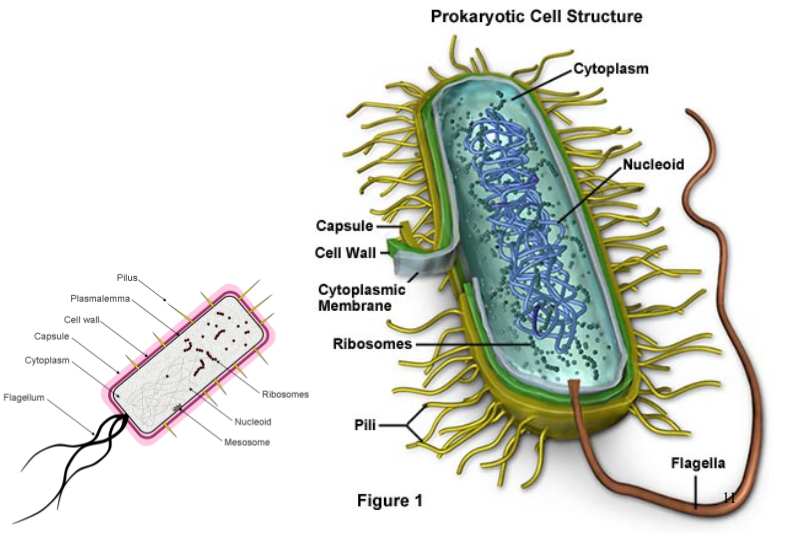
\includegraphics[width=0.6\textwidth]{prokaryotes}
\caption{Prokaryotic cell}
\label{Prokaryotic cell}
\end{figure}

\subsubsection{Eukaryotes}

This class is composed by all the remaining species (e.g. plants, animals, 
fungus, protist, etc). In this scenario, the cells contain organelles (e.g. 
mitochondria, cloroplasts in plants, Golgy system, lysosomes) and the DNA is 
stored into a compartment (i.e. nucleus and nucleolus).

\begin{figure}[!htpb]
\centering
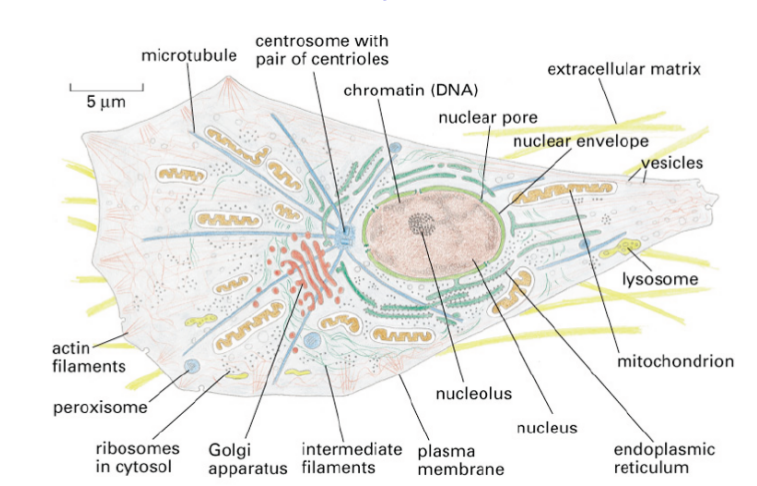
\includegraphics[width=0.6\textwidth]{eukaryotes}
\caption{Eukaryotic cell}
\label{Eukaryotic cell}
\end{figure}

\subsection{Phylogenetics - the tree of life}

Organisms are related through their evolutionary history, which can be traced 
using their genetic material.

\subsection{Multicellular organisms}

To build up a multicellular organisms, there are different steps. All start with 
a zygote cell, that start to divide and multiplicate. Once there are a lot of 
cells, they start to differentiate. In this way, the same basic cell can 
specialize for a specific task. At the end of this process, we obtain a mature 
organism.

\subsubsection{What makes a biological species?}

There are a lot of questions about biological species. Some of the most importants 
are:
\begin{itemize}
\item What is causing the difference between species?
\item How do species arise?
\item What is causing differences between members of the same population?
\end{itemize}

These important questions in biology are dealing with the `decoding' of information 
that resides in the genetic material. Differences in DNA (genotype, an organism's 
full hereditary information) lead to differences between members of the same 
species (phenotype, an organism's actual observed properties, such as morphology, 
development, or behavior).

\subsection{What makes us human?}

Let's have a look at our nearest neighbor: the chimpazee. There are differences 
in: gene expression\footnote{Khaitovich et al., `Evolution of primate gene 
expression,'Nature Rev. Genetics: Sept 2006 issue.} and duplication, `non-coding' 
sequences and several other events. Moreover, there are genes showing 
human-specific patterns (e.g. HAR1 in the brain).

\subsubsection{The human brain and the HAR1 gene}

Out of 35,000 non-coding genes, 49 candidate segments have evolved a lot in the 
human lineage. The most drastically altered of all is a segment dubbed HAR1 
(for human accelerated region 1). It is 118 base pairs long. Chimpanzees and 
chickens, separated by over 300 million years, carry versions of HAR1 that are 
identical except for two base pairs. In humans, on the other hand, 18 out of 
118 base pairs have changed since we split from chimps\footnote{Pollard et al. 
(2006) Nature 443, 167-172}.

Human cells make RNA molecules out of the HAR1 segment. Specifically, brain 
cells express HAR1 in the cortex, the hippocampus, and certain other regions. 
The sequence of HAR1 suggests that an RNA molecule produced from it would be 
stable enough to carry out some important job, such as regulating the activity 
of protein-coding genes. HAR1 probably plays several roles. It is not just 
active in the adult brain, but in development-guiding cells in the fetus.

HAR1, is part of a novel RNA gene (HAR1F) that is expressed specifically in 
Cajal-Retzius neurons in the developing human neocortex from 7 to 19 
gestational weeks, a crucial period for cortical neuron specification and 
migration. HAR1F is co-expressed with reelin, a product of Cajal-Retzius neurons
that is of fundamental importance in specifying the six-layer structure of the 
human cortex. HAR1 and the other human accelerated regions provide new candidates 
in the search for uniquely human biology. However, HAR1 is also active in the 
ovary and testis of adult humans. Perhaps selection has acted on HAR1 in connection 
with reproduction, rather than with thought, although expression of HAR1 is far 
smaller in the sex cells than in the brain. Still, it's a strange point that may
be worth raising at your next party: we have genes that are only active in our 
brains and sex cells.

However, recent evidence points at Biased Gene Conversion (BCG) to explain the 
divergence of HAC. BCG speeds up the rate of evolution in certain genes, and
increases the rate at which certain mutations spread through a population, 
regardless of whether they are beneficial or harmful. Since BGC can cause 
harmful mutations to spread through populations, many of the genetic changes 
leading to human-specific characters may be the result of the fixation of
(originally) harmful mutations. This contrasts the traditional Darwinistic view
that they are the result of natural selection in favour of adaptive mutations.

\subsubsection{Gene conversion}

It is a process by which DNA sequence information is transferred from one DNA 
helix (which remains unchanged) to another DNA helix, whose sequence is altered.
It is one of the ways a gene may be mutated. Gene conversion may lead to 
non-Mendelian inheritance.
